\section{DSP}
The \emph{OMAP3530} general purpose processor (from now on referred to as the
\emph{GPP}) contains a \emph{TMS320} digital signal processor (\emph{DSP}).This
core is optimised for using multiple calculation channels simultaneously: it is
a \emph{VLIW} (Very Long Instruction Word) processor that can utilise eight
functional units at the same time. More specifically, we can use six ALU's and
two multipliers per instruction. Another interesting feature is that each
multiplier can perform two 16 x 16-bit multiplications as well, giving us
potentially four multiplications in parallel.

The GPP unit has to first start up the DSP core, give it an executable to run
and afterwards detach the core as well. Furthermore, the requirements specified
that the matrices to multiply are generated on the GPP core as well (which is 
of course not a bad idea because the GPP is way more flexible: it can easily
be changed to read the matrices from a file or standard input, and we can
offload a part of the work to the GPP itself and also the \emph{NEON} as we 
will discuss later as well). 

\subsection{Communication}
This however brings us to one complication: the matrices have to be moved to
the DSP core, while the (partial) end result has to be sent back to the GPP.
Our first goal is thus to set up communications and send matrices back and forth
between the two cores. 

\begin{figure}[h]
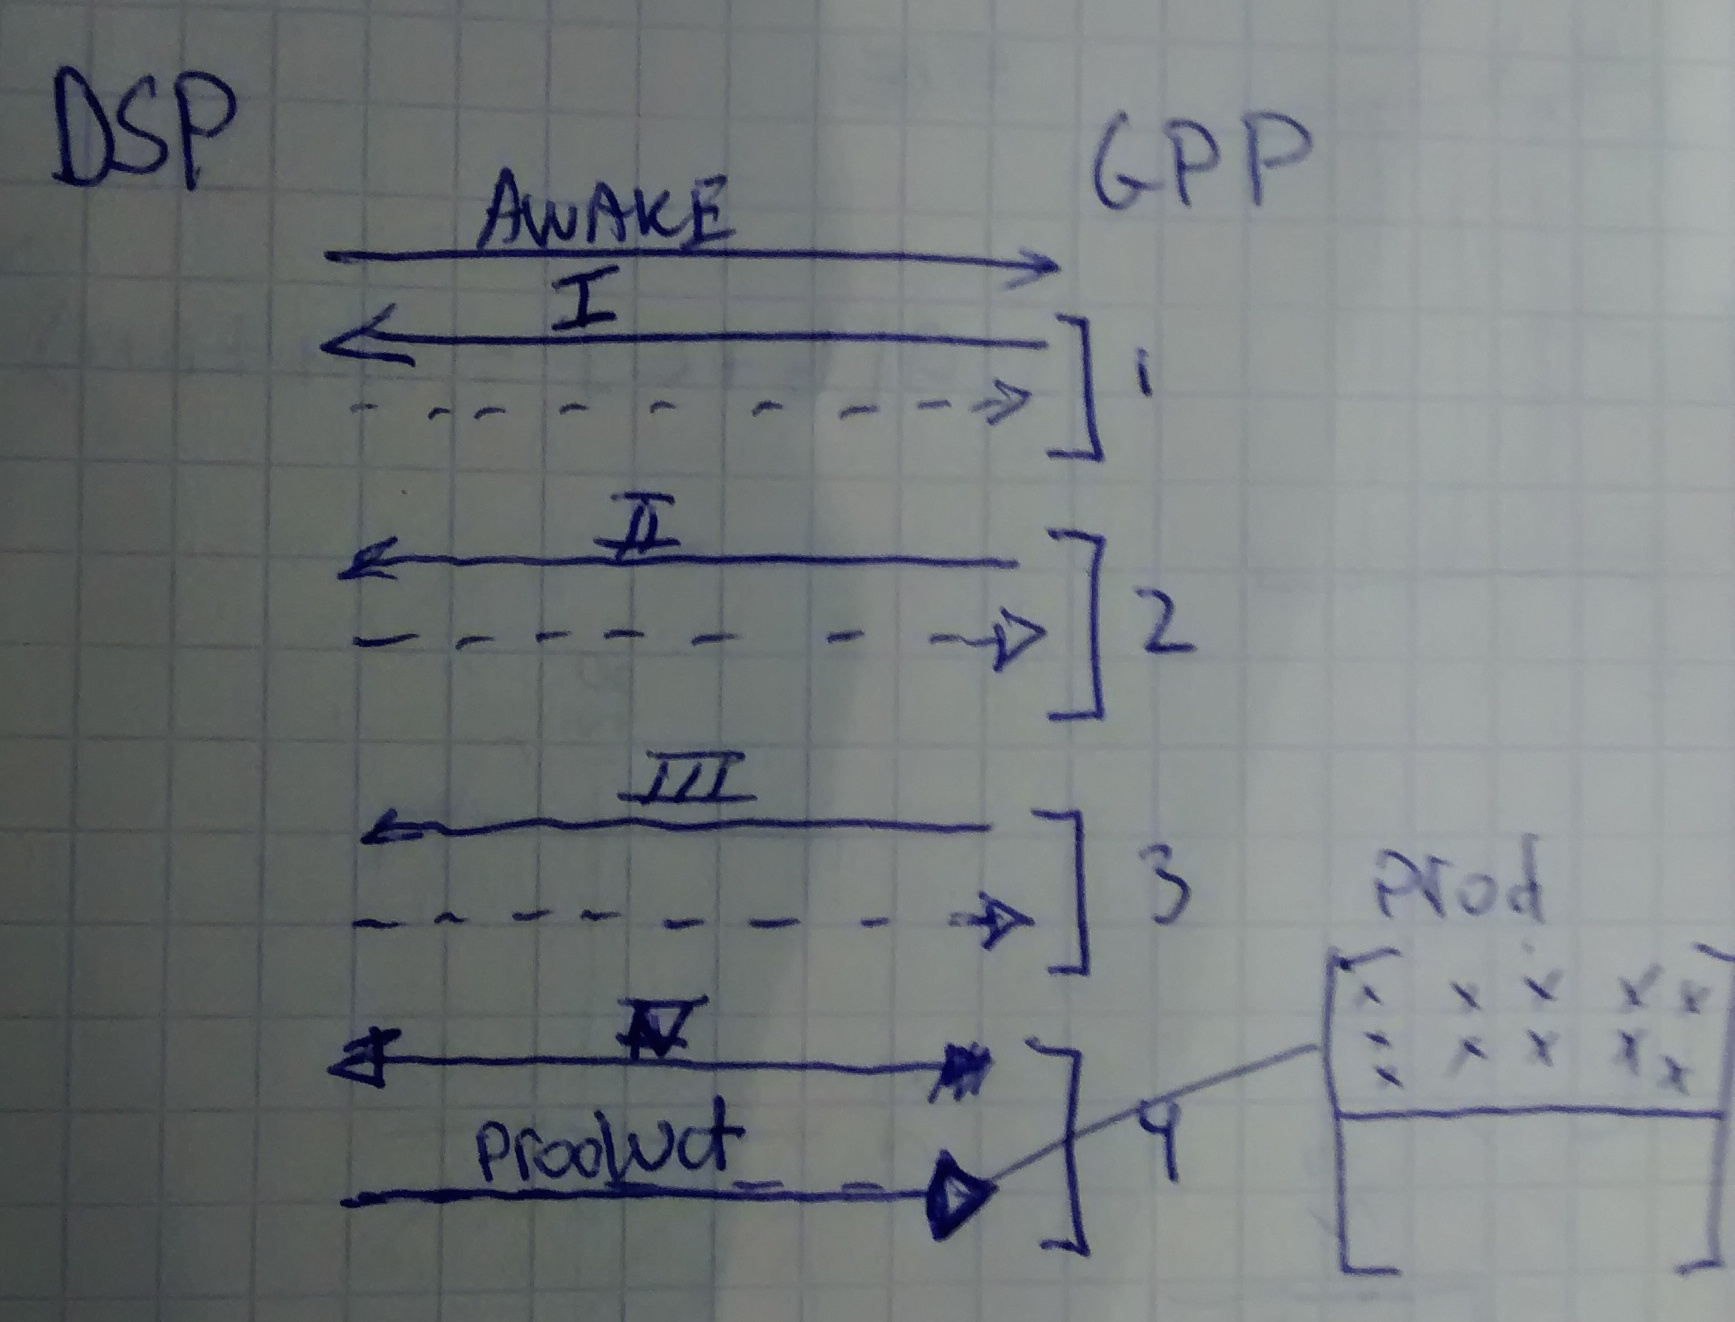
\includegraphics[width=\textwidth]{gpp_dsp_com}
\caption{Describing the communication process between the cores over time}
\label{fig:gpp_dsp_com}
\end{figure}

Unfortunately the communication API is slightly verbose and hard to handle.
For example, the sender has to allocate memory for a message, sends it and the
receiver has the possibility to send it back, or free the message. If we opted
for the latter and re-allocate every message we would always crash the DSP core.
The former option would mean that if we wanted to send more than one message
directly from the GPP, the DSP would have to send the entire message back first.
We however observed that the communication overhead is negligible, so we
decided to always re-use the same message. The general communication time-line
is described in figure~\ref{fig:gpp_dsp_com}. One observation in this time-line
is that we send data six times. The reason why will be discussed in the next
section.

\subsubsection{Message Format}
We used the existing reference communication implementation and it's message
structure, but we extended it with our own matrices and an extra field that
indicates how big the resulting matrix should be. One thing we had to do 
was determine the maximum matrix size we could assign, such that it would fit 
in one message. This message would be stored inside a section of
\emph{APP\_BUFFER\_SIZE} large, thus our message structure has to fit in there. 
We experimentally found that we could send up to around 90k bytes per message.

The source matrices are 16 bit, but the result should be at least 32 bits. 
To accommodate for both 
situations in the same control message structure while optimally using our
message in a uniform way, we opted to use a \emph{union} structure so we 
can either send two 16 bit matrices or one 32 bit matrix at a time. The 
structure is given in figure~\ref{code:control_msg}. 

Because we have to send up to $128*128*2*2=65.536$ (2 matrices of 16 bits)
bytes from the GPP to the DSP, we need at least four messages considering
our bandwidth limit of 90k bytes. Thus we send the source in four messages, 
each containing a quarter of both matrices. The DSP only calculates a half of
the result matrix, making two messages sufficient: this results in six 
communication steps.

\begin{figure}[h]
\begin{lstlisting}[language=C]
struct mat2x16 {
	int16_t mat1[SIZE][SIZE];
	int16_t mat2[SIZE][SIZE];
};

struct mat32 {
	int32_t mat1[SIZE][SIZE];
};

typedef union {
	struct mat2x16 m16;
	struct mat32 m32;
} mat_t;

#define ARG_SIZE 256
typedef struct ControlMsg
{
    MSGQ_MsgHeader header;	// 20 bytes
    Uint16 command;				// 2 bytes
    Char arg1[ARG_SIZE];		// 256 bytes
    Uint8 size;					// 1 byte
    mat_t mat;						// 4 * SIZE * SIZE bytes
} ControlMsg;
\end{lstlisting}
\caption{The message structure we used}
\label{code:control_msg}
\end{figure}
